\chapter{Introduction}
\label{chapter:intro}

Thin liquid films appear in our daily life in multiple forms. 
Many of this forms are not even recognized by us.
Of course I hope to explain this in a more detailed manner throughout this thesis but first let me draw a picture.

During the time I spend researching thin liquid films with the lattice Boltzmann method I had to learn the governing equations of fluid dynamics. 
Those equations are called the Navier-Stokes equations and they resemble the dynamics of system constraint due to several symmetries~\cite{Navier, Stokes}.
Solving this equations in a strict mathematical manner, which means showing existence and smoothness of a solutions, is an elusive quest. 
This fact is nicely displayed that although this equations are around for roughly two centuries they are still one of the six unsolved ''Millenium problems''.
Nevertheless with the constant innovation in computing techniques and computing hardware it is possible to \textit{brute force} an approximate solution for a large class of problems.
The thin film equation is based on the Navier-Stokes equations but admits a crucial simplification due to a dimensional reduction~\cite{ReynoldsLubr}.

Such I had to learn and understand a lot of equations and even more so learn about algorithms and numerical techniques, especially the lattice Boltzmann method (LBM)~\cite{doi:10.1146/annurev.fluid.30.1.329, PhysRevE.56.6811, PhysRevE.65.046308}.
Now this picture of sitting in front of a monitor, constantly reading and coding, have little to do with how great and tangible the field of thin liquid film research is.
Whenever some liquid advances on a yet dry surface we can observe a thin film flow, drinking from a glass of water or painting fresh canvas. 
On the other hand watching rain drops run down a window can as well be described by the thin film equation. 
Why drops form at all after a foggy morning can be studied in the framework of the thin film equation as well.
Although these phenomena happen in many situations their theoretical understanding is far from being complete.
Just to highlight one of the above mentioned situations, the wetting of a dry surface.
However mad this sounds theoretically this process can not be explained.
Even worse to move liquid on top of dry surface would need an infinite amount of energy.
This has to do with the so called contact line and is called the ''Huh-Scriven paradox''~\cite{HUH197185}.
Of course nature finds a way around that issue and I hope that this manuscript will help to understand what a contact line is and why it moves.

Following will be of course the introduction of the mathematical model with its partial differential equation. 
However this is nothing more than a rather efficient way of describing the problem.
Strictly speaking mathematics as well as algorithm serve as a tools not as the goal. 
Therefore I try my best to keep it as simple as possible with analogies and self explaining pictograms.

\section{Thin Film Applications}
\label{section:applications}

\section{Literature Overview}
\label{section:literature}
Theory concerning lubrication is as old as the Navier-Stokes equations. 
Osborn Reynolds was the first to deduce the lubrication approximation~\cite{ReynoldsLubr} already in 1886.

\section{Outline}
\label{section:outline}



% \begin{figure}[h!]
% \centering
% 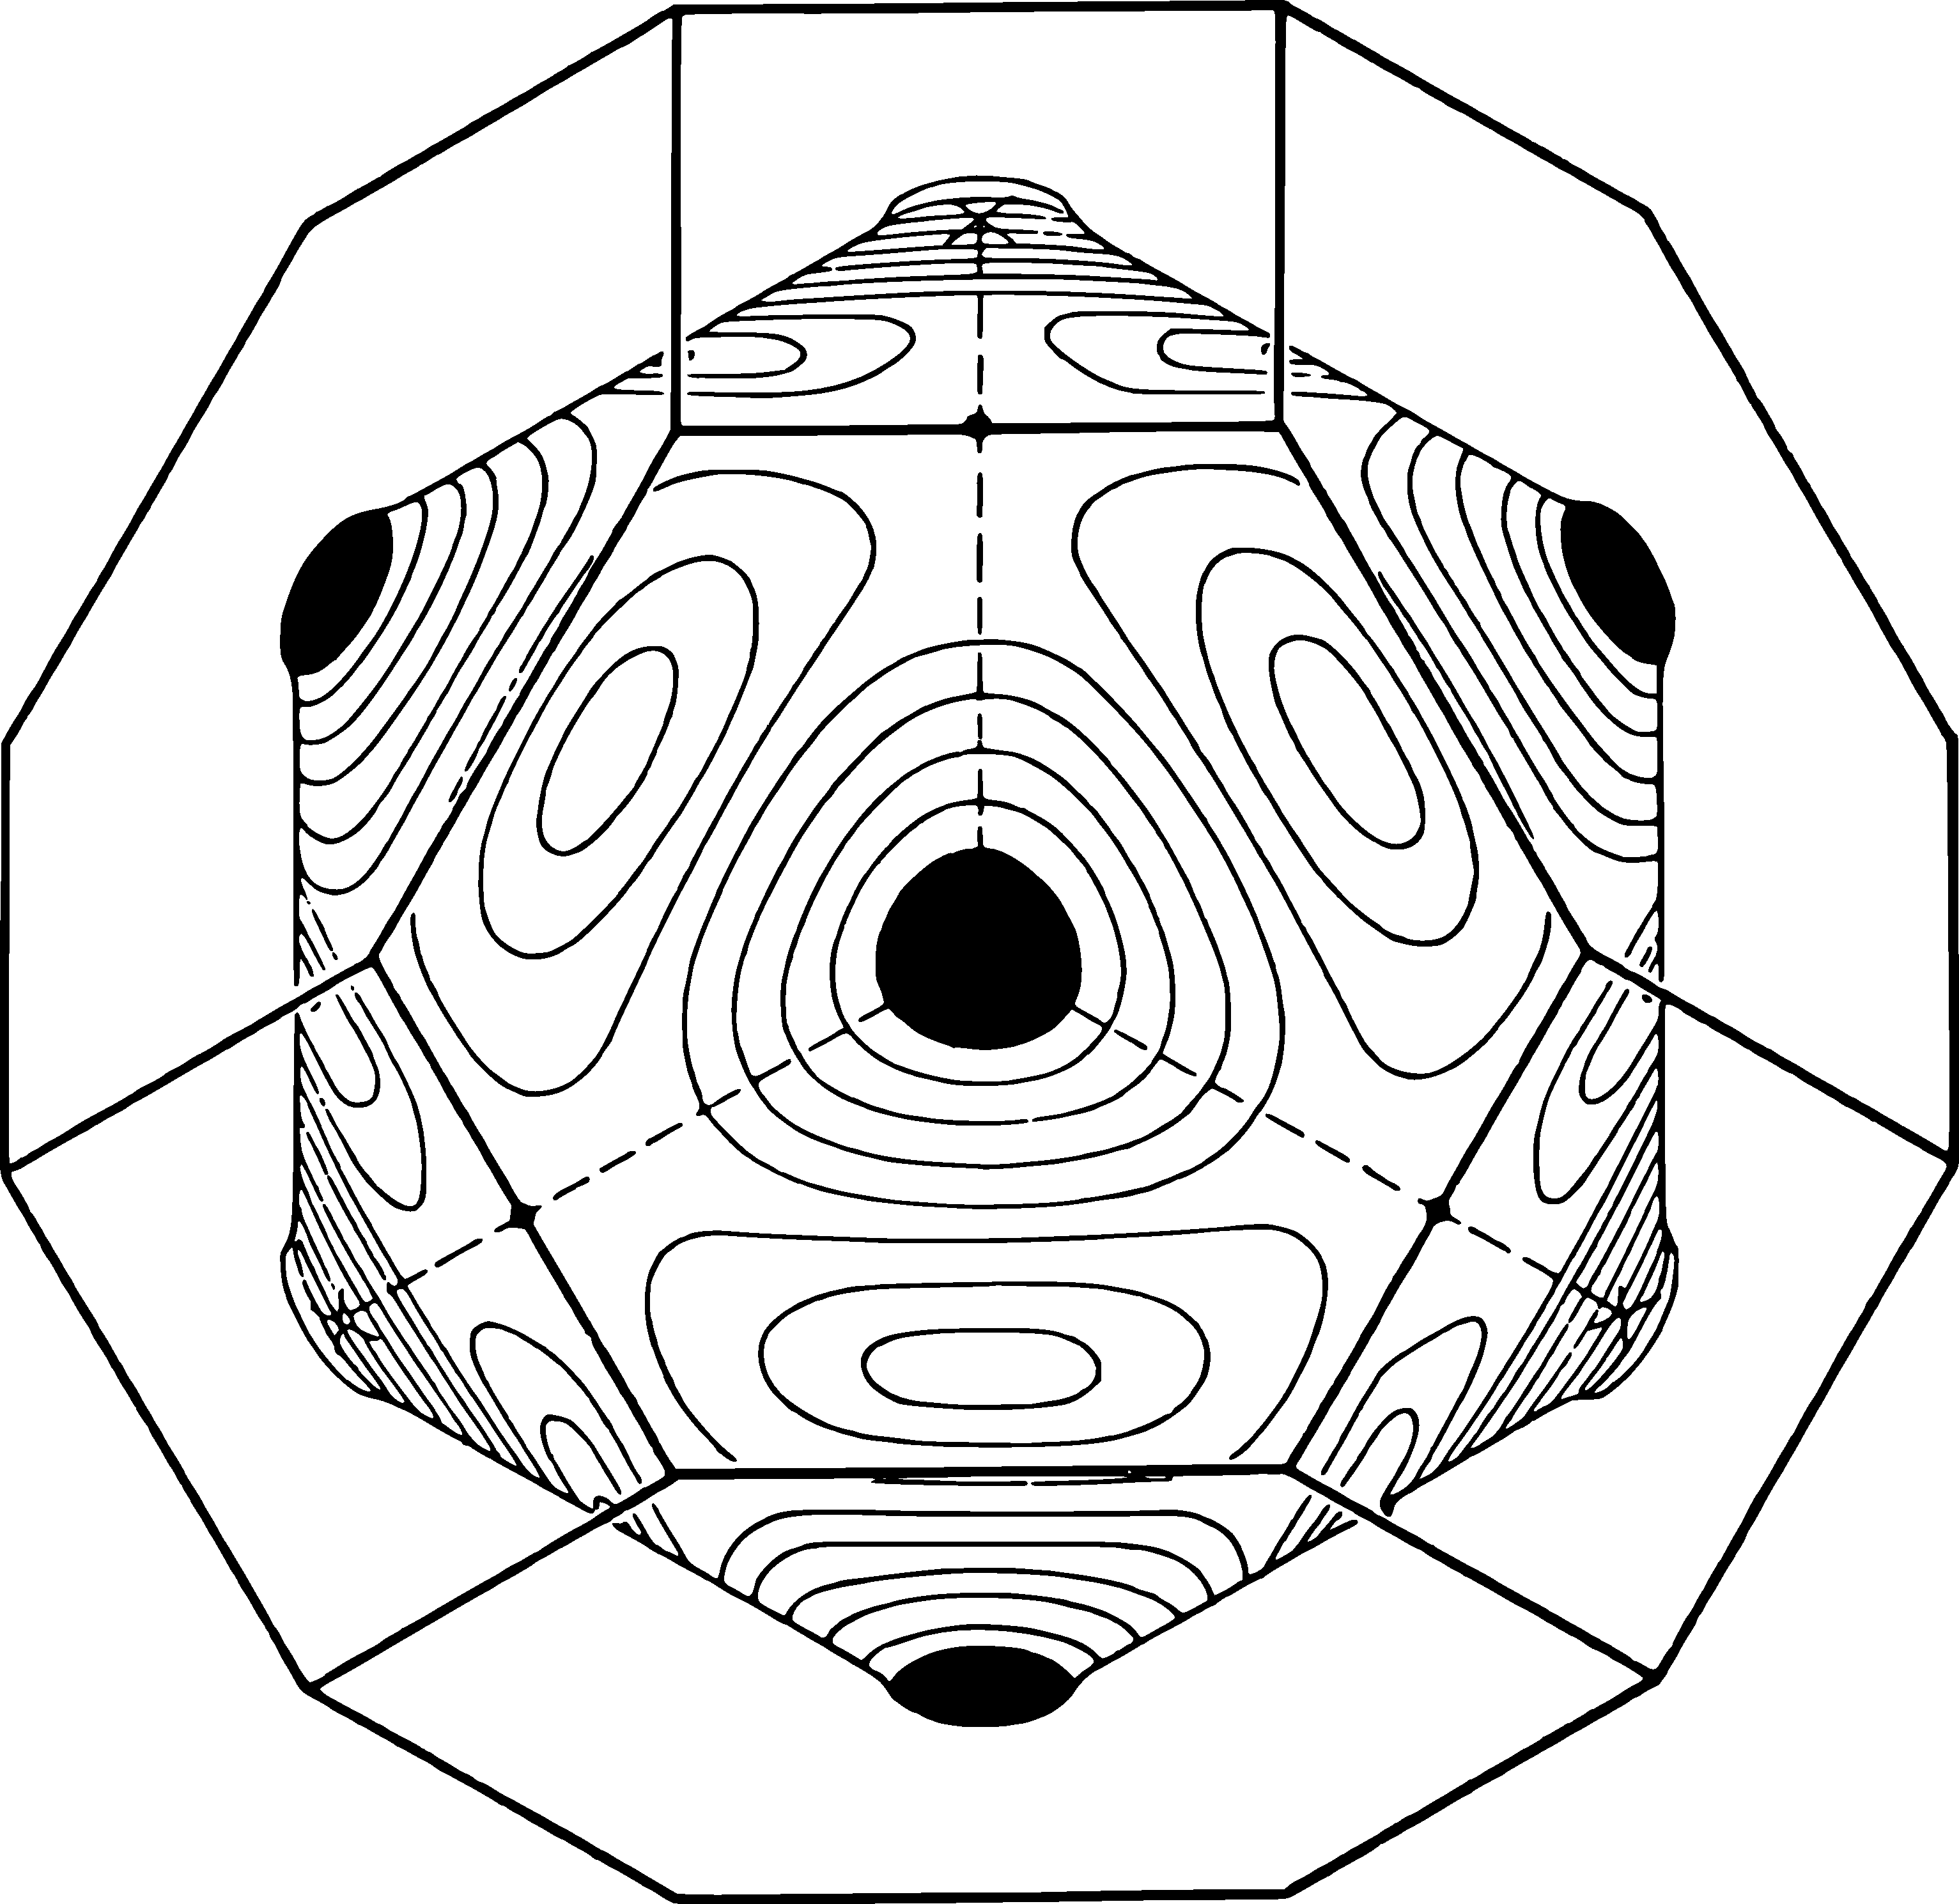
\includegraphics[width=0.45\textwidth]{graphics/fermi_copper_pippard}%
% \caption[Isosurface von Kupfer nach Pippard]{Isosurface von Kupfer nach Pippard \cite{Pippard1957}}%
% \label{fig:fermi_copper_pippard}%
% \end{figure}